\chapter{\textbf{\Large ANNEXES}}

\newpage

\section{Installation des Machines Virtuelles}

\subsection{Installation d'une Debian Minimale}
\paragraph{}
Ce chapitre va présenter l'installation d'une machine virtuelle sous le système d'exploitation Debian. Nous vous proposons de suivre une installation minimale, sans connexion réseau.

\begin{figure}[h]
\centering
 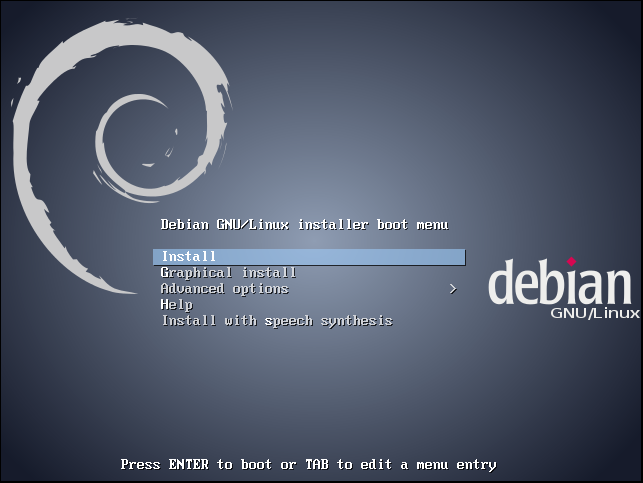
\includegraphics[scale=0.5]{img/install/Deb_inst_1.png}
 \caption{Ecran d'accueil pour l'installation de Debian}
\end{figure}
\begin{figure}[h]
 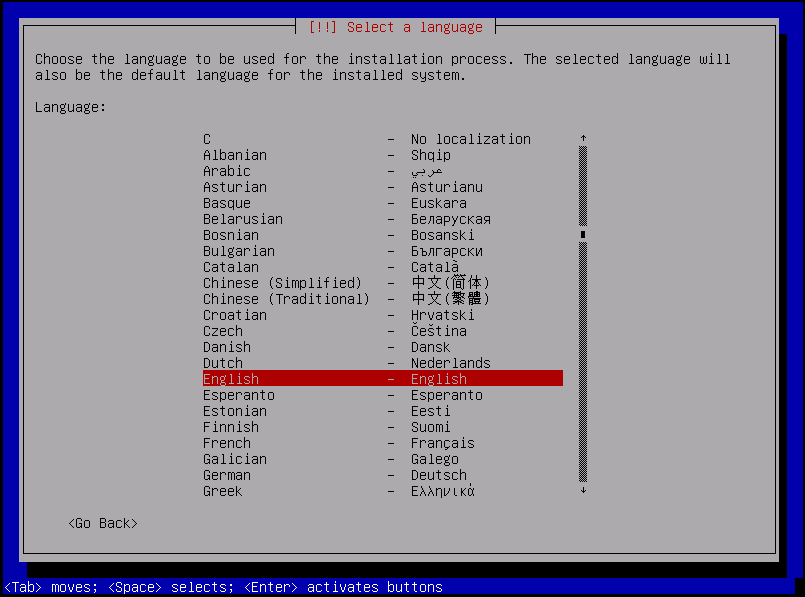
\includegraphics[scale=0.35]{img/install/Deb_inst_2.png}
 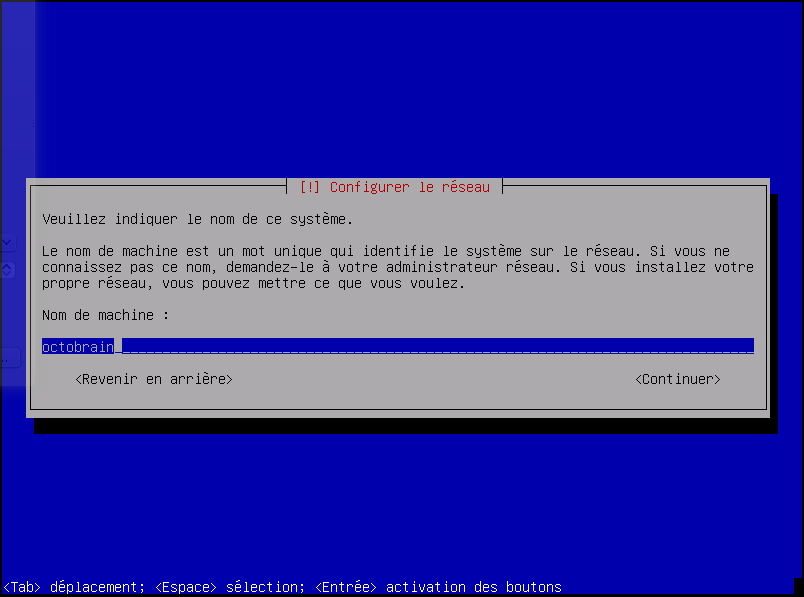
\includegraphics[scale=0.35]{img/install/Deb_inst_5.png}
 \caption{Choix de la langue et configuration réseau}
 \end{figure}
\begin{figure}
 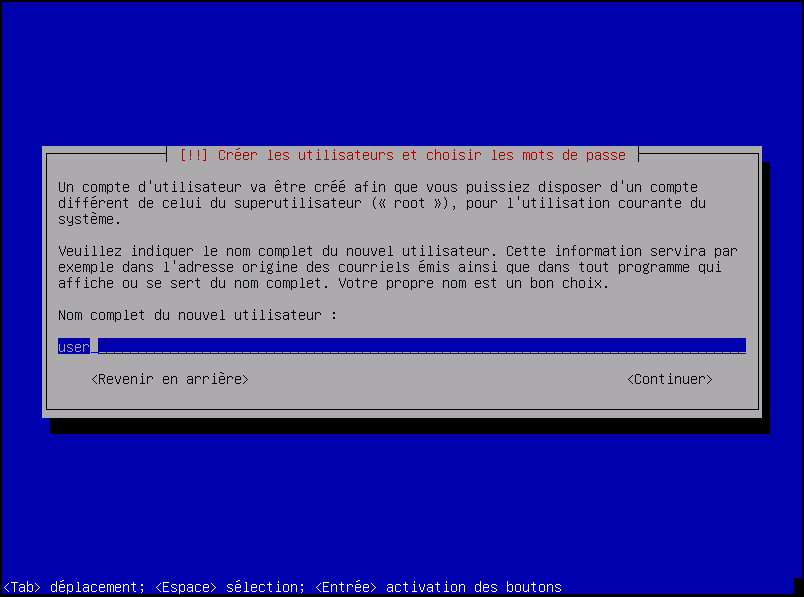
\includegraphics[scale=0.35]{img/install/Deb_inst_7.png}
 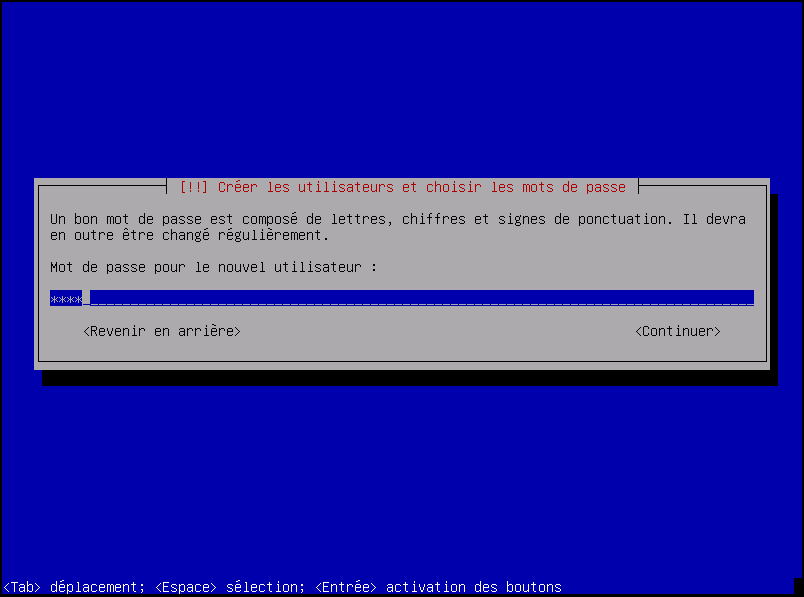
\includegraphics[scale=0.35]{img/install/Deb_inst_8.png}
 \caption{Création d'un utilisateur avec son mot de passe}
\end{figure}
\begin{figure}
 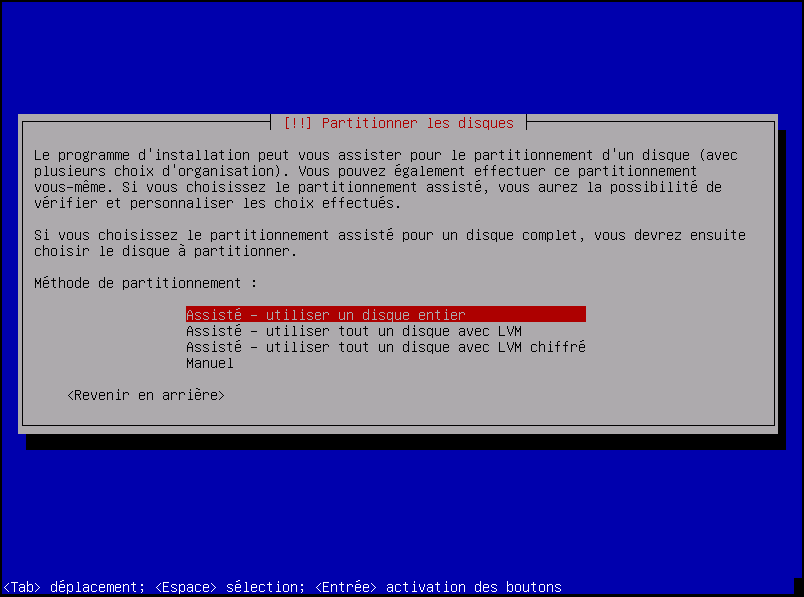
\includegraphics[scale=0.35]{img/install/Deb_inst_9.png}
 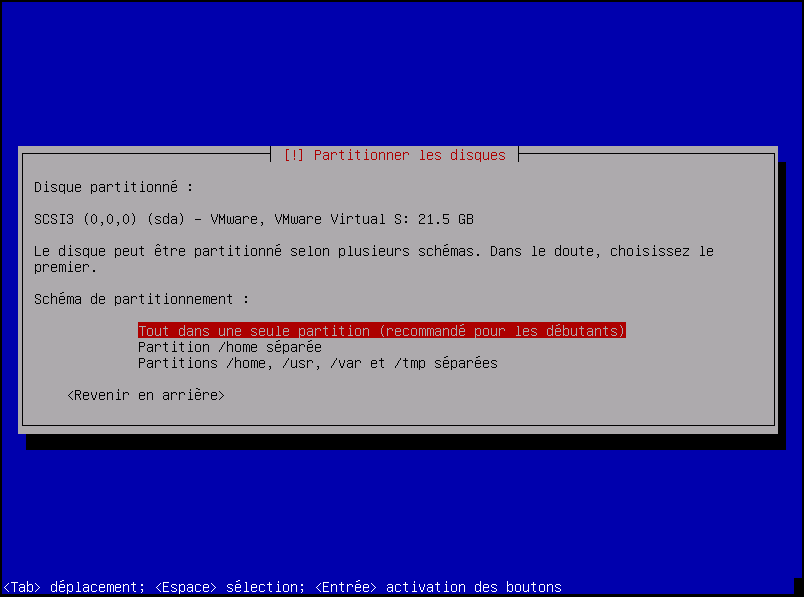
\includegraphics[scale=0.35]{img/install/Deb_inst_11.png}
 \caption{Partitionnement du disque dur et choix d'emplacement d'installation}
\end{figure}
\begin{figure}
 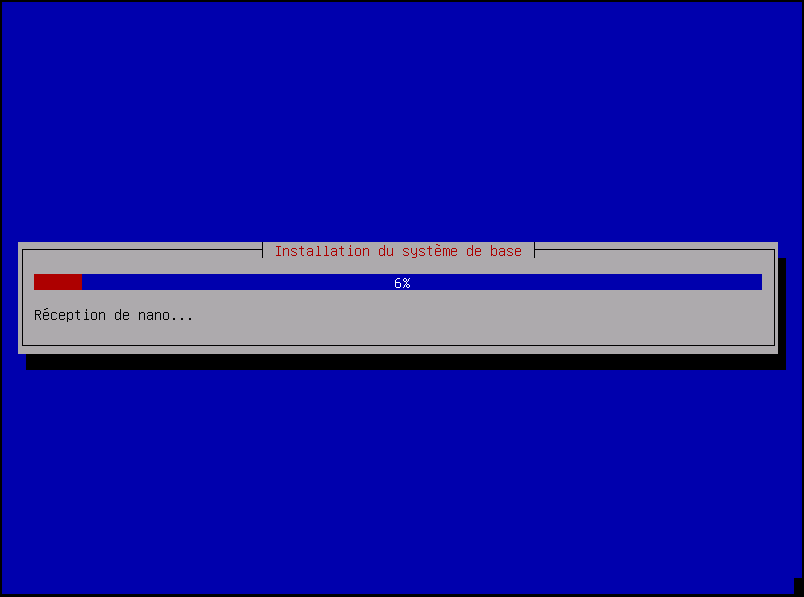
\includegraphics[scale=0.35]{img/install/Deb_inst_13.png}
 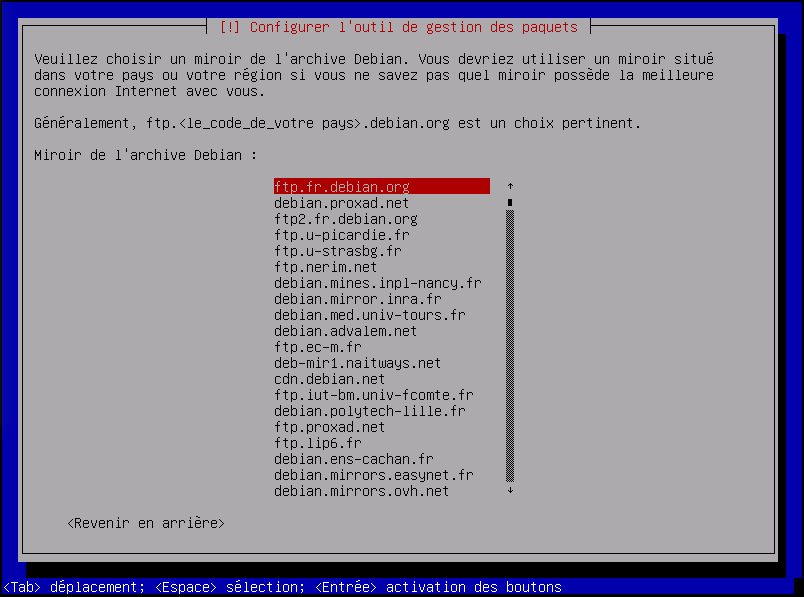
\includegraphics[scale=0.35]{img/install/Deb_inst_14.png}
 \caption{Installation du système et configuration des miroirs de packets}
\end{figure}
\begin{figure}
 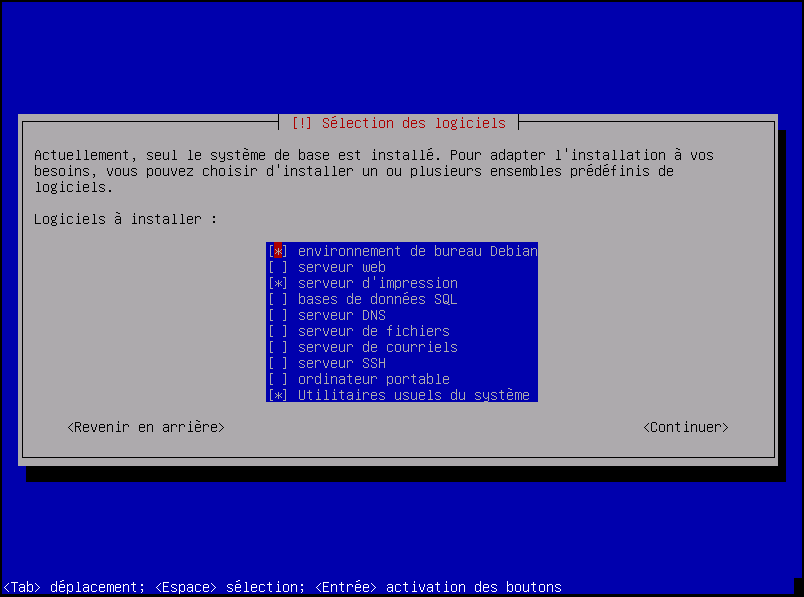
\includegraphics[scale=0.35]{img/install/Deb_inst_15.png}
 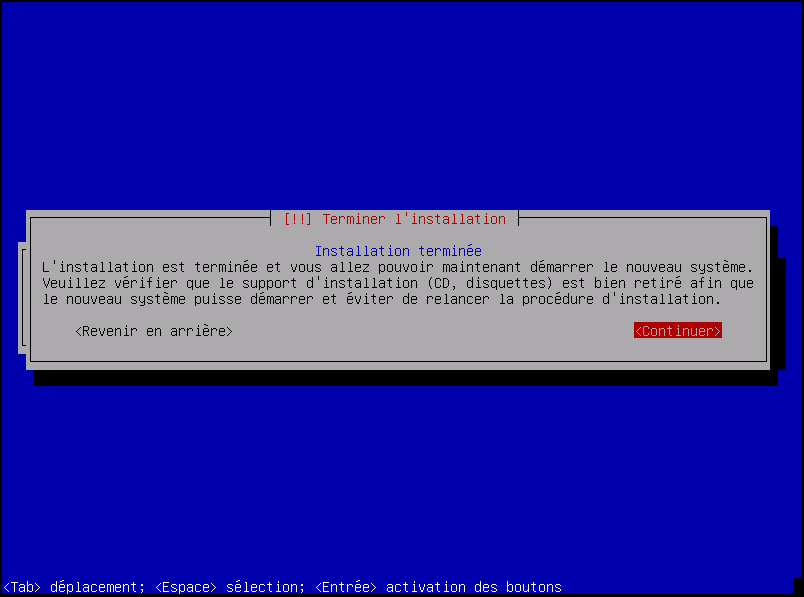
\includegraphics[scale=0.35]{img/install/Deb_inst_16.png}
 \caption{Choix des logiciels importants et finalisation de l'installation}
\end{figure}
\begin{figure}[h]
\centering
 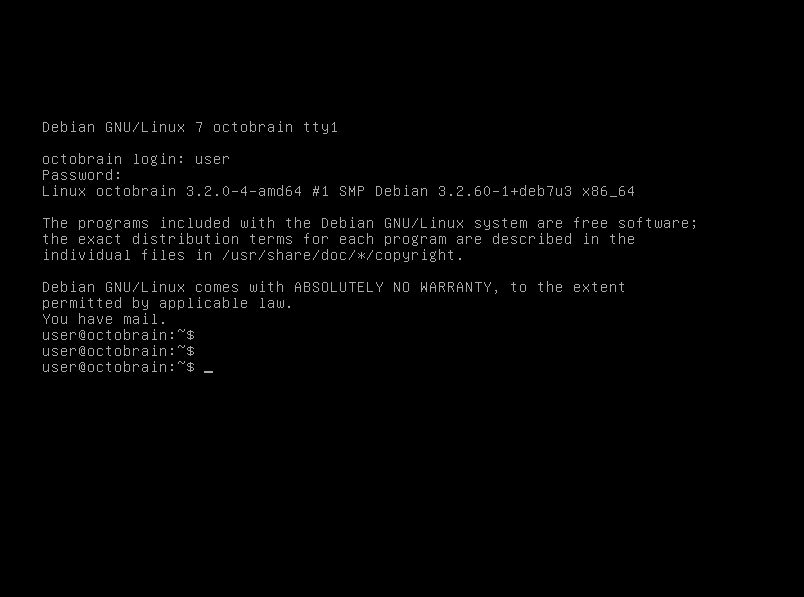
\includegraphics[scale=0.5]{img/install/Deb_inst_17.png}
 \caption{Ecran du système fonctionnel}
\end{figure}

\paragraph{}
Nous avons maintenant une machine virtuelle fonctionnant avec Debian 7 en installation minimale. C'est-à-dire que seul les packages essentiels sont installés. 
Afin de faire fonctionner correctement Octopus Supervisor, il faut ajouter les paquets suivants : gcc, make, libssl-dev, libsqlite3-dev.


\subsection{Installation d'un Xubuntu}
\paragraph{}
Nous allons vous montrer ci-dessous les différentes étapes d'une installation graphique du système Xubuntu.

\begin{figure}[h]
 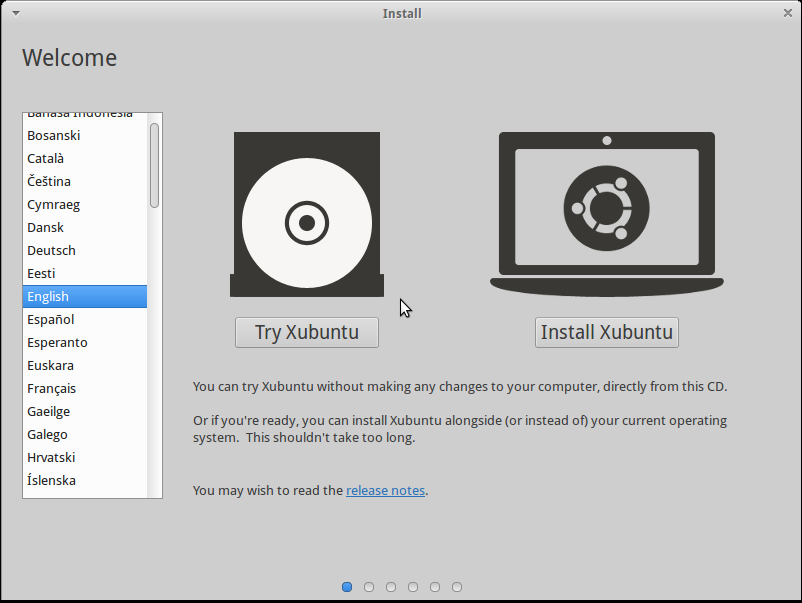
\includegraphics[scale=0.38]{img/install/Xub_inst_1.png}
 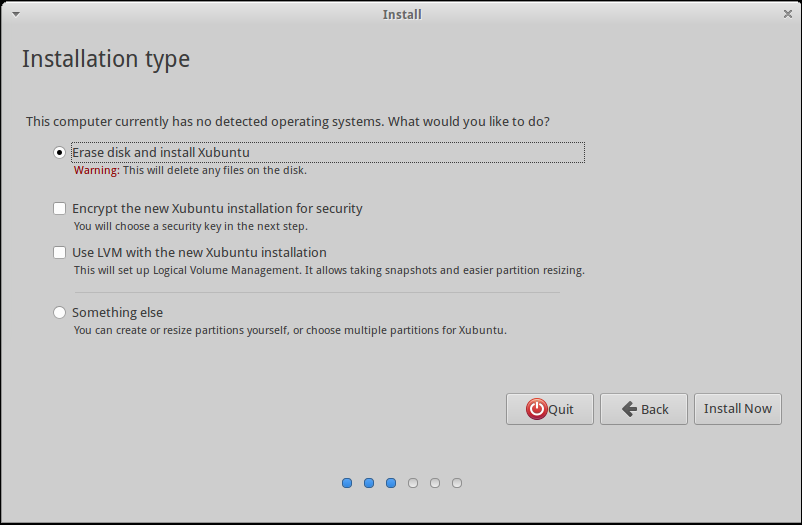
\includegraphics[scale=0.38]{img/install/Xub_inst_2.png}
 \caption{Choix de la langue et du type d'installation}
 \end{figure}
 \begin{figure}[h]
 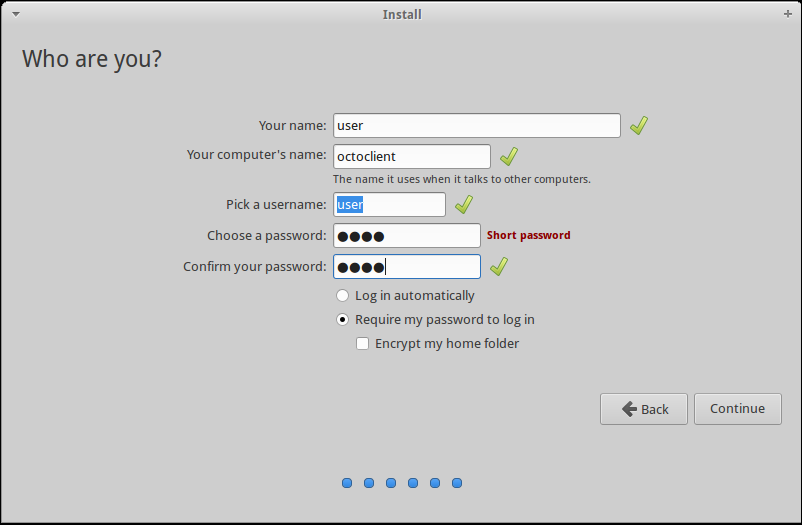
\includegraphics[scale=0.38]{img/install/Xub_inst_3.png}
 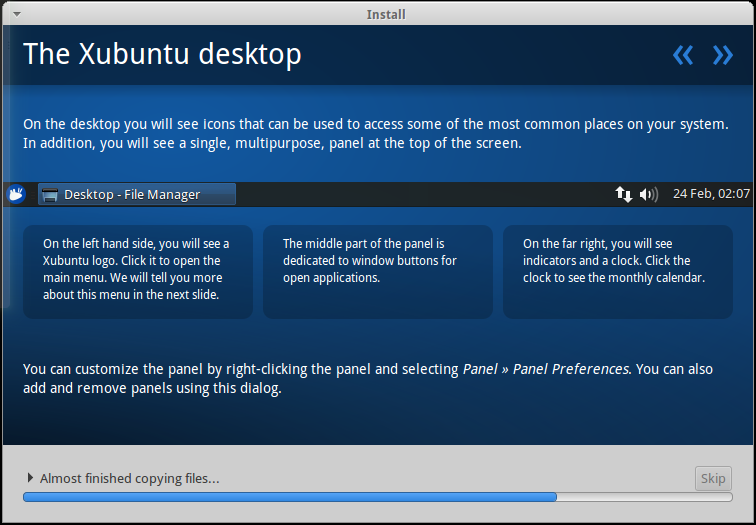
\includegraphics[scale=0.38]{img/install/Xub_inst_4.png}
 \caption{Définition d'un utilisateur et installation du système}
 \end{figure}
 \begin{figure}[h]
 \centering
 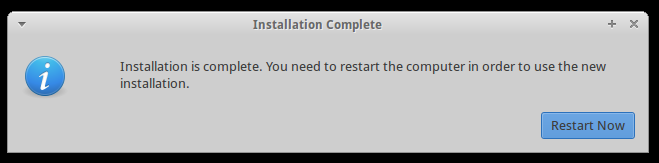
\includegraphics[scale=0.5]{img/install/Xub_inst_6.png}
 \caption{Fin de l'installation}
 \end{figure}
 \begin{figure}[h]
 \centering
 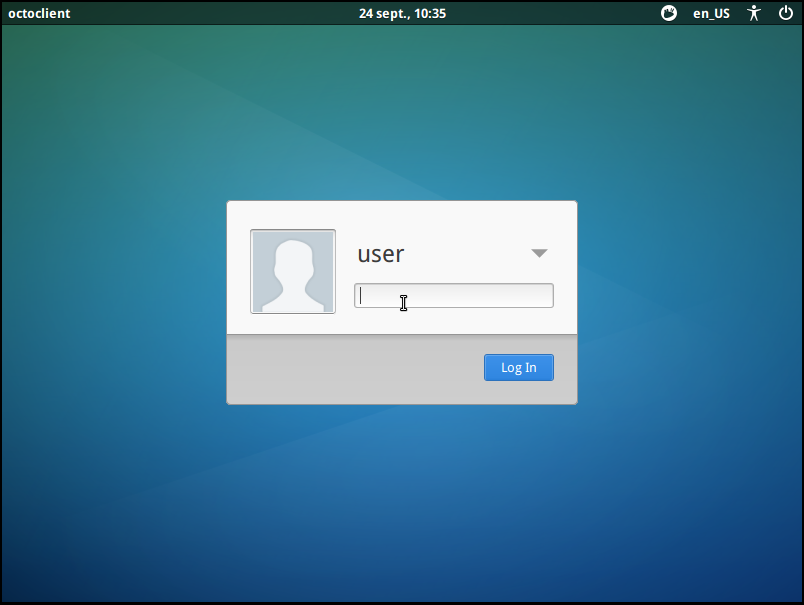
\includegraphics[scale=0.5]{img/install/Xub_inst_7.png}
 \caption{Ecran de connexion utilisateur}
 \end{figure}
 
 \paragraph{}
 Maintenant, nous avons un client opérationnel sous Xubuntu. Et nous pouvons ensuite installer le paquet client d'Octopus Supervisor.
 